\documentclass[oneside, final, 14pt]{article}
\usepackage[utf8]{inputenc}
\usepackage[russianb]{babel}
\usepackage{vmargin}
\setpapersize{A4}
\setmarginsrb{2cm}{1.5cm}{1cm}{1.5cm}{0pt}{0mm}{0pt}{13mm}
\usepackage{indentfirst}
\usepackage{graphicx}
\usepackage{amsmath}
\usepackage{amssymb}
\usepackage{amsthm}
\usepackage {titlesec}
\usepackage{algorithm}
\usepackage{algpseudocode}
\bibliographystyle{unsrt} 
%\usepackage{biblatex}
\begin{document}
\sloppy
	\renewcommand\contentsname{Содержание} %%% renaming the Table of Contents
%	\renewcommand\chaptername{}
%	\renewcommand\chapternum{}
%	\thispagestyle{empty}

\begin{titlepage}
\begin{center}
\bfseries
Московский Государственный Университет \\имени М.~В.~Ломоносова\\
Факультет вычислительной математики и кибернетики\\
Кафедра математической физики\\

\includegraphics[width=0.4\textwidth]{msu_logo_small.png}\\
\vfill	

\mdseries
\begin{Large}
КУРСОВАЯ РАБОТА СТУДЕНТА 402 ГРУППЫ\\
\end{Large}
Турганбаева Сатбека Амангельдыулы\\
\vfill	
Тема курсовой работы:\\
\vspace{1cm}
\bfseries
\begin{Large}
""\\
\end{Large}
\vfill	

  \begin{flushright}
        Научный руководитель:\\
        д.ф-м.н. профессор Разгулин~А.~В.
    \end{flushright}

\vfill	


\end{center}

\begin{center}
	Москва 2017
\end{center}

\end{titlepage}

\tableofcontents

\newpage
\section{Введение}
Системы адаптивной оптики используемые в современных телескопах используют гибкие зеркала, для коррекции аберраций, вызванных турбулентность атмосферы Земли. Одним из устройств для измерения волнового фронта является датчик Шака-Гартмана. Данный датчик измеряет градиент волнового фронта, вместо него самого. Получаются матрицы градиентов $X$ и $Y$.

В \cite{new_method1} был предложен метод восстановления волнового фронта по его наклонам с использованием преобразования Хаара. Идея метода заключается в том, что наклоны волнового фронта могут быть представлены в виде суперпозиции сверток с фильтрами преобразования Хаара. Используя это соотношение возможно выполнить "замену переменной", и получить разложение волнового фронта по вейвлетам Хаара. Затем, применив стандартный алгоритм обратного преобразования получить исходный волновой фронт. Стоит отметить, что в \cite{new_method1} кроме наклонов волнового фронта и его интенсивности также требовалась и интенсивность правого нижнего квадранта $_{HH}^{M-1}\Phi$ , но в более новой статье \cite{new_method2} было предложено более простое решение, и ослаблены требования к начальным данным. 

Целью работы является ознакомление с методом , его программная реализация, а также реализация средств для его дальнейшего исследования. В ходе работы были разобраны статьи \cite{new_method1}- \cite{new_method2}, и на их основе написана первая часть работы, знакомящая с преобразованием Хаара и методом. При программной реализации был написан ряд модулей, реализующих как сам метод, так и средства для его исследования. В работе описан их функционал. Также приведены примеры работы метода на полиномах Цернике.
\newpage
\section{Преобразование Хаара} 
\subsection{Формулировки и определения}
\textbf{Z-преобразованием} дискретного сигнала $\{s_j\}_{ j \in Z}$ называется полином Лорана 
$P_{s}(z) = \sum_{j \in Z} s_{j}z^{-j}$.

$h = (\frac{1}{\sqrt{2}}, \frac{1}{\sqrt{2}}),~g = (\frac{1}{\sqrt{2}}, -\frac{1}{\sqrt{2}})$ - низкочастотный и высокочастотный фильтры преобразования Хаара.

$$ H_{L}(z) = \frac{1 + z^{-1}}{\sqrt{2}} $$
$$ H_{H}(z) = \frac{1 - z^{-1}}{\sqrt{2}} $$
$H_{L}(z)$,~$H_{H}(z)$ - z - преобразования фильтров $h$ и $g$ соответственно.

\textbf{Линейной сверткой} двух дискретных сигналов $a(n),~ n=0 \ldots N-1$ и $b(n),~ n=0 \ldots M-1$ называется выражение:
$$ h = a \otimes b $$
$$ h(n) =  \sum_{m=0}^{n} a(m)b(n-m) $$
В ввиду того, что сигналы конечномерные на границах возникает неопределенность из-за отсутствия соответствующих элементов. Проблема решается различными способами: дополнение одного из обоих сигналов $0$-ми, константами, симметричное отражение и т.д.

Также одним из свойств $z$-преобразования является то, что $z$-преобразование свертки двух сигналов равно произведению $z$-преобразований этих сигналов. 

\textbf{$\uparrow s$} - операция, добавляющая $0$ после каждого элемента сигнала $s$.

\textbf{$\downarrow_k s$} - операция, удаляющая каждый $k$-ый элемент сигнала $s$.

Если $s = (1,2,3,4)$, то $\uparrow_2 s = (1,0,2,0,3,0,4,0)$, а $\downarrow_{2} s = (1,3)$.

Также стоит отметить, что:
$$\downarrow_2 H_L(z^{2^k}) = H_L(z^{2^{k-1}}),~ k\geq 2$$
$$\downarrow_2 H_H(z^{2^k}) = H_H(z^{2^{k-1}}),~ k\geq 2$$
$$\uparrow_2 H_L(z^{2^{k-1}}) = H_L(z^{2^{k}}),~ k\geq 2$$
$$\uparrow_2 H_H(z^{2^{k-1}}) = H_H(z^{2^{k}}),~ k\geq 2$$

В дальнейшем под сигналом будет пониматься его $z$-преобразование и наоборот.
\subsection{Одномерный сигнал}
Будем предполагать в дальнейшем, что размерность сигналов равна $2^m,~m \geq~1$.

Свернем сигнал $h_m(z)$, $dim~h_m = 2^m$ с фильтрами $H_L(z)$,~$H_H(z)$, а затем применим к получившемуся операцию $\downarrow_2$.

Получим сигналы: $$h_{L_{m-1}}(z) = \downarrow_2 \{h_m(z)H_L(z)\}$$ $$h_{H_{m-1}}(z) = \downarrow_2 \{h_m(z)H_H(z)\}.$$ Их размерности будут в два раза меньше,размерности исходного сигнала $h_m$.

$h_{L_{m-1}}(z)$ называется низкочастотной составляющей сигнала $h_m$, a $h_{H_{m-1}}(z)$ высокочастотной. 

Восстановление исходного сигнала происходит так:
$$h_m(z) = \uparrow_2 \{ h_{L_{m-1}}(z) \} H_L(z) + \uparrow_2 \{ h_{H_{m-1}}(z) \} H_H(z)	$$
Описанные выше преобразования выполняют один шаг прямого и обратного преобразования Хаара. Прямое преобразование называется анализом, обратное синтезом.

Если положить, что $h_m = h_{L_m}$, то алгоритм анализа выглядит так:
\begin{algorithm}
\caption{Алгоритм анализа}
\begin{algorithmic}
	\For{$k=1 \ldots m$}
	\State $h_{L_{m-k}}(z) = \downarrow_2 \{h_{L_{m-k+1}}(z)H_L(z)\}$
	\State $h_{H_{m-k}}(z) = \downarrow_2 \{h_{L_{m-k+1}}(z)H_H(z)\}.$
	\EndFor
\end{algorithmic}
\end{algorithm}


$k$ называется разрешением разложения. Анализ будет происходить до тех пор, пока не останется один элемент.
\begin{algorithm}[H]
\caption{Алгоритм синтеза}
\begin{algorithmic}
	\For{$k=m \ldots 1$}
		\State$h_{L_{m-k + 1}}(z) = \uparrow_2 \{ h_{L_{m-k}}(z) \} H_L(z^{-1}) + \uparrow_2 \{ h_{H_{m-k}}(z) \} H_H(z^{-1})$
	\EndFor
\end{algorithmic}
\end{algorithm}	

\subsection{Дополнение нулями}
В описываемом методе при анализе будем дополнять нулями справа, а при синтезе слева. Ниже приведены примеры анализа и синтеза сигнала $(1,2,3,4)$. Для наглядности используется нестандартные пары фильтров, $[1,1]$, $[1,-1]$ и $[0.5,0.5]$, $[0.5,-0.5]$.
\begin{center}
\center{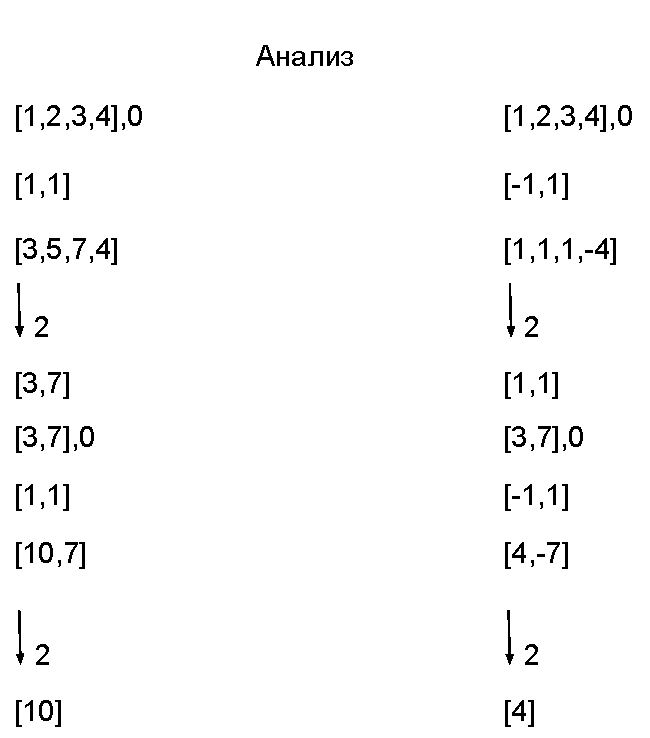
\includegraphics[width=0.6\linewidth]{analyze.pdf}}
\center{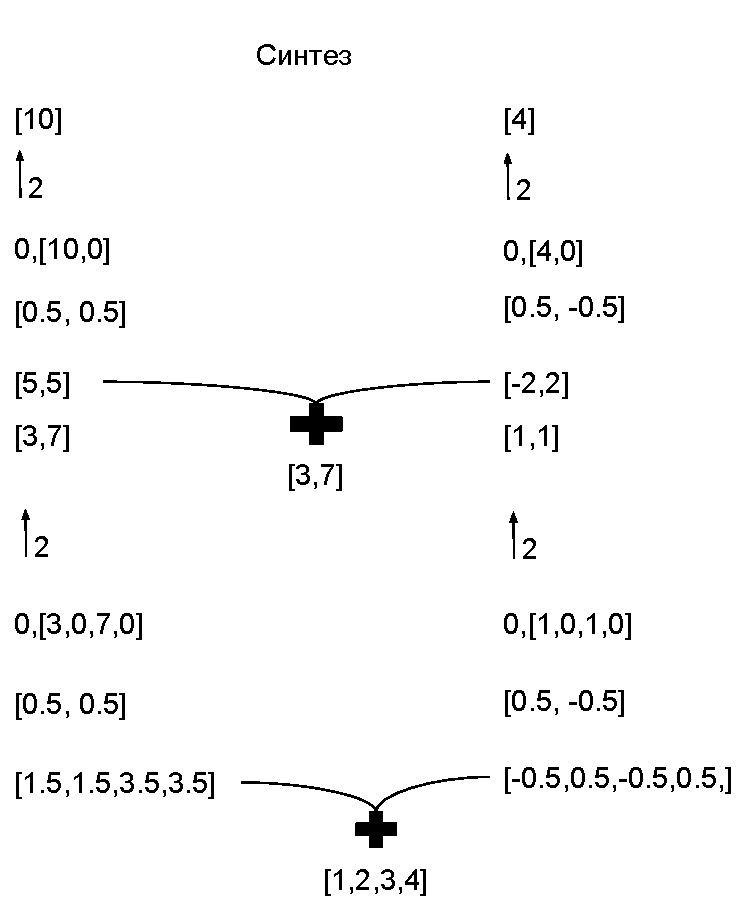
\includegraphics[width=0.6\linewidth]{synthesis.pdf}}
\end{center}


\subsection{Двумерное преобразование}
Пусть дана матрица $^{M}\Phi, ^{M}\Phi \in \mathbb{R}^{2^{M}\times2^{M}}$. Применим к каждой строке матрицы один шаг анализа. В результате получим матрицы $_L^{m-1}\Phi$, $_H^{m-1}\Phi$. К каждому столбцу обеих матриц также применим шаг анализа. В итоге получим четыре матрицы $_{LL}^{m-1}\Phi$, $_{LH}^{m-1}\Phi$, $_{HL}^{m-1}\Phi$, $_{HH}^{m-1}\Phi$. $_{LL}^{m-1}\Phi$ - является низкочастотной составляющей двумерного сигнала, остальные три матрицы содержат детализирующую информацию. Таким образом будет выполнен первый шаг двумерного преобразования Хаара. Нужно проделать аналогичные операции с $_{LL}^{m-1}\Phi$ для следующего шага. Такми образом, шаг двумерного преобразования свелся к композиции одномерных преобразований.

Синтез происходит аналогичным образом: в обратном анализу порядке дополняется нулями соответствующая размерность и применяются фильтры Хаара, а затем результаты складываются.

Пусть $^{M}\Phi = _{LL}^{M}\Phi$
\begin{algorithm}[H]
\caption{Алгоритм 2D-анализа}
\begin{algorithmic}
	\For{$k=M \ldots 1$}
		\State $_{LL}^{k-1}\Phi = \downarrow_{2}$ $\{_{LL}^{k}\Phi H_{L}(z_h)H_{L}(z_v)\}$
		\State $_{LH}^{k-1}\Phi = \downarrow_{2}$ $\{_{LL}^{k}\Phi H_{L}(z_h)H_{H}(z_v)\}$
		\State $_{HL}^{k-1}\Phi = \downarrow_{2}$ $\{_{LL}^{k}\Phi H_{H}(z_h)H_{L}(z_v)\}$
		\State $_{HH}^{k-1}\Phi = \downarrow_{2}$ $\{_{LL}^{k}\Phi H_{H}(z_h)H_{H}(z_v)\}$
	\EndFor
\end{algorithmic}
\end{algorithm}
\begin{algorithm}[H]
\caption{Алгоритм 2D-синтеза}
\begin{algorithmic}
	\For{$k=1 \ldots M$}
	\State  $_{LL}^{k-1}\Phi=$ $\uparrow_2$  $\{_{LL}^{k-1}\Phi H_L(z_v^{-1}) + _{LH}^{k-1}\Phi H_L(z_v^{-1})\}H_L(z_h^{-1})+ $ $\uparrow_2$ $\{_{HL}^{k-1}\Phi H_L(z_v^{-1}) + _{HH}^{k-1}\Phi H_L(z_v^{-1})\}H_H(z_h^{-1})$
	\EndFor
\end{algorithmic}
\end{algorithm}	
Полученное $2$-$D$ разложение можно представить в виде диаграммы, где на каждом уровне $LL$, $LH$, $HL$ и $HH$ составляющим соответствуют определенные квадранты. 
\begin{center}
\center{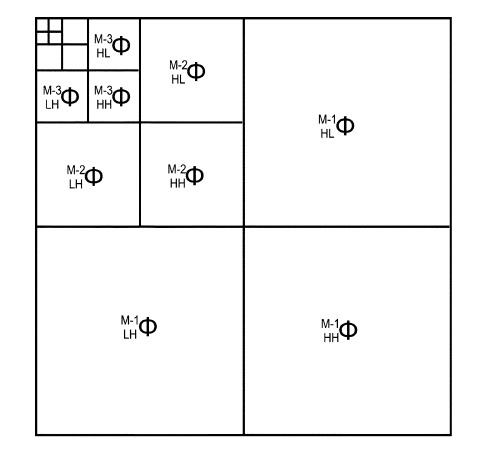
\includegraphics[width=0.6\linewidth]{hwaf_decomp.png}}
\end{center}
\subsection{Явные формулы для анализа}
Из алгоритма анализа непосредственно выводятся формулы для $LL$, $LH$, $HL$ и $HH$ составляющих на каждом уровне.
\begin{equation}\label{LL}
_{LL}^{M-m}\Phi=
\downarrow_{2^m} \{^M\Phi\prod\limits_{k = 0}^{m-1} H_L(z_h^{2^k})
							\prod\limits_{k = 0}^{m-1} H_L(z_v^{2^k})\}
\end{equation}
\begin{equation}\label{LH}
_{LH}^{M-m}\Phi=
\downarrow_{2^m} \{^M\Phi H_H(z_v^{2^{m-1}}) \prod\limits_{k = 0}^{m-1} H_L(z_h^{2^k})
							\prod\limits_{k = 0}^{m-2} H_L(z_v^{2^k})\}
\end{equation}
\begin{equation}\label{HL}
_{HL}^{M-m}\Phi=\downarrow_{2^m} \{^M\Phi H_H(z_h^{2^{m-1}}) \prod\limits_{k = 0}^{m-2} H_L(z_h^{2^k})
						\prod\limits_{k = 0}^{m-1} H_L(z_v^{2^k})\}
\end{equation}
\begin{equation}\label{HH}
_{HH}^{M-m}\Phi=\downarrow_{2^m} \{^M\Phi H_H(z_v^{2^{m-1}}) H_H(z_v^{2^{m-1}}) \prod\limits_{k = 0}^{m-2} H_L(z_h^{2^k})
							\prod\limits_{k = 0}^{m-2} H_L(z_v^{2^k})\}
\end{equation}
\newpage
\section{Градиенты. Геометрия Хаджина и Фрайда}
\subsection{Геометрия Хаджина и Фрайда}
В адаптивной оптике используются два различных способа представления наклонов волнового фронта. Согласно \cite{how}
это геометрии Хаджина и Фрайда.
Геометрия Хаджина:
$$_{H}x_{i,j}=-\phi_{i,j}+\phi_{i,j+1}$$
$$_{H}y_{i,j}=-\phi_{i,j}+\phi_{i+1,j}$$
Получившиеся матрицы $_H^{M}X$, $_H^{M}Y$ имеют размерности $2^M \times(2^M - 1)$ и $(2^M - 1) \times 2^M$ соответственно.
Геометрия Фрайда:
$$_{F}x_{i,j}=\frac{_{H}x_{i,j} + _{H}x_{i+1,j}}{2} = \frac{-\phi_{i,j}+\phi_{i,j+1}-\phi_{i+1,j}+\phi_{i+1,j+1}}{2}$$
$$_{F}y_{i,j}=\frac{_{H}y_{i,j} + _{H}y_{i,j+1}}{2} = \frac{-\phi_{i,j}-\phi_{i,j+1}+\phi_{i+1,j}+\phi_{i+1,j+1}}{2}$$
Получившиеся матрицы $_F^{M}X$, $_F^{M}Y$ имеют одинаковые размерности $2^M - 1 \times 2^M - 1$.
\subsection{Градиенты и преобразование Хаара}
Справедливы следующие соотношения.
\begin{equation}\label{_H^MX}
_H^MX = ^M\Phi\sqrt{2}H_H(z_h) 
\end{equation}
\begin{equation}\label{_H^MY}
_H^MY = ^M\Phi\sqrt{2}H_H(z_v)
\end{equation}
\begin{equation}\label{_F^MX}
_F^MX = \frac{_H^MX H_L(z_v)}{\sqrt{2}}=^M\Phi H_H(z_h) H_L(z_v)
\end{equation}
\begin{equation}\label{_F^MY}
_F^MY = \frac{_H^MY H_L(z_h)}{\sqrt{2}}=^M\Phi H_L(z_h) H_H(z_v)
\end{equation}
\newpage
\section{Вывод формул прямого преобразования}
Рассмотрим случай, когда известны вертикальные и горизонтальные наклоны, а также интенсивность волнового фронта. Иначе говоря имеются: $_F^MX$, $_F^MY$, $_H^MX$, $_H^MY$ , $_0^{LL}\Phi$.

Необходимо получить из имеющихся данных получить $2D$-разложение волнового фронта, а затем восстановить сам волновой фронт, применив к полученному разложению стандартный алгоритм синтеза.\cite{new_method1}
Диаграмма разложения которое необходимо получить будем аналогична диаграмме стандартного разложения:
\begin{center}
\center{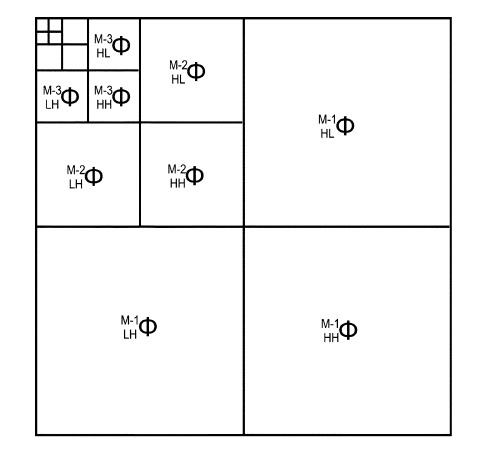
\includegraphics[width=0.6\linewidth]{hwaf_decomp.png}}
\end{center}
Отличаться будут лишь формулы (\ref{LL})-(\ref{HH}). "Идейно" метод заключается в замене переменной. Используя соотношения (\ref{_H^MX})-(\ref{_F^MY}), получим аналоги (\ref{LL})-(\ref{HH}).
\subsection{Получение LH, HL квадрантов}
Из соотношений (\ref{_H^MX}), (\ref{_H^MY}) и (\ref{HL}), (\ref{LH}) соответственно, непосредственно вытекает, что:
\begin{center}

$ 	_{HL}^{M-1}\Phi = \downarrow_{2}$ $ _F^MX $ 

$ 	_{LH}^{M-1}\Phi = \downarrow_{2}$ $ _F^MY $

\end{center}

Докажем справедливость выражения $H_{H}(z^{2^{m-1}}) = \sqrt{2}^{m-1} H_H(z) \prod \limits_{k=0}^{m-2} H_L(z^{2^k})$
\begin{proof}
Запишем $H_{H}(z^{2^{m-1}})$ в виде полинома
$$H_{H}(z^{2^{m-1}}) = \frac{1 - z^{2^{m-1}}}{\sqrt{2}}$$
$$\frac{1 - z^{2^{m-1}}}{\sqrt{2}} = \frac{(1-z^{2^{m-2}})(1+z^{2^{m-2}})}{\sqrt{2}}=\ldots=\frac{(1-z)(1+z)(1+z^2)\ldots(1+z^{2^{m-2}})}{\sqrt{2}}$$
$$H_{H}(z^{2^{m-1}}) = \sqrt{2}^{m-1} H_H(z) \prod \limits_{k=0}^{m-2} H_L(z^{2^k})$$
\end{proof}

\textbf{LH, $m>1$:}

\[
_{LH}^{M-m}\Phi=
\downarrow_{2^m} \{^M\Phi [H_H(z_v^{2^{m-1}})] [\prod\limits_{k = 0}^{m-1} H_L(z_h^{2^k})]
							\prod\limits_{k = 0}^{m-2} H_L(z_v^{2^k})\}=\]
							
\[
=\downarrow_{2^m} \{^M\Phi [\sqrt{2}^{m-1} H_H(z_v) \prod \limits_{k=0}^{m-2} H_L(z_v^{2^k})]
					[H_L(z_h)\prod \limits_{k=1}^{m-1} H_L(z_h^{2^k})]
					\prod\limits_{k = 0}^{m-2} H_L(z_v^{2^k})
\}			
\]
\[
=\sqrt{2}^{m-1} \downarrow_{2^m} \{^M\Phi H_L(z_h) H_H(z_v)\prod \limits_{k=1}^{m-1} H_L(z_h^{2^k})\prod \limits_{k=0}^{m-2} H_L^2(z_v^{2^k})
\]
\[
=\sqrt{2}^{m-1} \downarrow_{2^m} \{_F^MY \prod \limits_{k=1}^{m-1} H_L(z_h^{2^k})\prod \limits_{k=0}^{m-2} H_L^2(z_v^{2^k})
\]
\textbf{HL, $m>1$:}

Выводится аналогично, LH
\[_{HL}^{M-m}\Phi=
\sqrt{2}^{m-1} \downarrow_{2^m} \{_F^MY \prod \limits_{k=0}^{m-2} H_L^{2}(z_h^{2^k})\prod \limits_{k=1}^{m-1} H_L(z_v^{2^k})\}
\]

\subsection{Получение HH квадранта}
\textbf{HH, $m=1$:}\cite{new_method2}

Докажем, что $_{HH}^{M-1}\Phi\downarrow_2 \{\frac{\sqrt{2}}{4}[_{H}^MX H_H(z_v) + _{H}^MY H_H(z_h)]\}$
%$_{HH}^{M-1}\Phi = \downarrow_2$ $ [^{M}\Phi H_H(z_h)H_H(z_v)]$
\begin{proof}
Известно, что $_{HH}^{M-1}\Phi = \downarrow_2$ $ [^{M}\Phi H_H(z_h)H_H(z_v)]$.

Распишем \begin{math} _{HH}^{M-1}\Phi = \downarrow_2 \{ \frac{\sqrt{2}}{2}\sqrt{2} ~^{M}\Phi H_H(z_h)H_H(z_v) \} \end{math}, выделив из (\ref{_F^MX}) $_H^MX$ получим:
\[
 _{HH}^{M-1}\Phi = \downarrow_2 \{\frac{\sqrt{2}}{2} ~_{H}^MX H_H(z_v)\} = \downarrow_2 \{\frac{\sqrt{2}}{4}2 ~_{H}^MX H_H(z_v)\}
\]

Разделив (\ref{_F^MX}) на (\ref{_F^MY}) получим:
\[
_{H}^MX H_H(z_v) = _{H}^MY H_H(z_h)
\]
Отсюда получим:
\[
_{HH}^{M-1}\Phi\downarrow_2 \{\frac{\sqrt{2}}{4}[_{H}^MX H_H(z_v) + _{H}^MY H_H(z_h)]
\]
\end{proof}

\textbf{HH, $m>1$:}
\[
_{HH}^{M-m}\Phi=\downarrow_{2^m} \{^M\Phi H_H(z_v^{2^{m-1}}) H_H(z_v^{2^{m-1}}) \prod\limits_{k = 0}^{m-2} H_L(z_h^{2^k})
							\prod\limits_{k = 0}^{m-2} H_L(z_v^{2^k})\}=\]
							
\[
=\downarrow_{2^m} \{^M\Phi \sqrt{2}^{m-1} H_H(z_h) \prod \limits_{k=0}^{m-2} H_L(z_h^{2^k})   
\prod \limits_{k=0}^{m-2} H_L(z_h^{2^k}) H_H(z_v^{2^{m-1}})H_L(z_v) \prod \limits _{k=1}^{m-2}H_L(z_v^{2^k})=
  \}
\]
\[
=\sqrt{2}^{m-1} \downarrow_{2^m} \{_F^MX \prod \limits_{k=0}^{m-2} H_L^2(z_h^{2^k}) H_H(z_v^{2^{m-1}}) \prod \limits_{k=1}^{m-2}H_L(z_v^{2k})    \}
\]
\newpage
\section{Программная реализация}
Программная реализация представляет из себя две группы модулей на языке Python 3.6. 

Первая группа реализует сам метод и предоставляет функции \textit{analyze} и \textit{syntesis}. Вторая группа отвечает за реализацию интерфейса для дальнейшего изучения метода.

Рассмотрим подробнее структуру первой группы модулей.

\subsection{Программная реализация метода}
Список группы модулей, реализующих сам метод:
\begin{itemize}
\item \textbf{data.py}
\item \textbf{gradients.py}
\item \textbf{measurements.py}
\item \textbf{util.py}
\item \textbf{decomposition.py}
\end{itemize}

\textbf{data.py} - модуль отвечает за задание начальных данных. Предоставляет функцию\textit{get\_plane}, которая задает сетку размера $2^M \times 2^M$ для дальнейших вычислений.

\textbf{gradients.py} - модуль предоставляет функции для нахождения градиента от заранее известной матрицы. В модуле находятся функции: \textit{Fried\_gradient\_model} и \textit{Hudgin\_gradien\_model}, которые возвращают градиенты по геометриям Фрайда и Хаджина.

\textbf{measurements.py} - модуль предоставляет функции для нахождения метрик схожести изображений.
Модуль включает функцию \textit{mse}, которая находит средне квадратичное отклонение двух изображений.

\textbf{util.py} - служебный модуль, используемый другими. Предоставляет функции для свертки сигналов, работы с $z$-преобразованиями. Включает в себя функции:
\begin{itemize}
\item  \textit{downsample} - реализует операцию $\downarrow_k$ c одномерными и двумерными массивами
\item \textit{convolve\_2d} - осуществляет свертку двумерного массива с фильтром либо по строкам, либо по столбцам;
\item \textit{GetH\_h} - возвращает вектор, соответствующий $z$-преобразованию $H_H(z^k)$, для $k         \geq 1$.
\item \textit{GetH\_l} - возвращает вектор, соответствующий $z$-преобразованию $H_L(z^k)$, для $k  \geq 1$.
\end{itemize}

\textbf{decomposition.py} - реализуется разложение двумерного сигнала по вейвлетам Хаара.
Основными функциями являются \textit{analyze} и \textit{syntesis} - именно они реализуют прямое и обратное преобразования Хаара. Ввиду того, что уже существует крупная библиотека, реализующая вейвлет преобразования \textbf{pywt (PyWawelets)}, результат функции \textit{analyze} не конфликтует с результатом библиотечной функции \textit{pywt.dwt2}, реализующей прямые вейвлет преобразования двумерных сигналов. В виду того, что в методе используется стандартный алгоритм обратного преобразования Хаара функция \textit{syntesis}, реализующая его является оберткой над библиотечной функций \textit{pywt.idwt2}.

\subsection{Программная реализация интерфейса для исследования метода}
Интерфейс для исследования метода реализуется двумя модулями \textbf{research.py} и \textbf{view.py}.

\textbf{research.py} используя модули из другой группы, предоставляет функции, которые возвращают информацию необходимую для исследования метода. Модуль предоставляет функцию \textit{get\_all}.

\textit{get\_all(func, grad\_x, grad\_y, x\_s, x\_e, y\_s, y\_e, M)}

Функция принимает в качестве параметров три функции: исходную функцию и два её градиента в явном виде, затем функция принимает параметры для задания сетки , на которой будут заданы функция и ее градиенты. Функция вычисляет следующий набор данных:
\begin{itemize}
\item исходную функцию
\item исходные градиенты
\item $_H^MX$, $_H^MY$ составляющие от градиента
\item $_F^MX$, $_F^MY$ составляющие от градиента
\item $LL$, $LH$, $HL$, $HH$ квадранты разложения
\item среднеквадратичное отклонение исходной функции от восстановленной ($LL[M]$)
\item размерность матрицы, M
\end{itemize}

\textbf{view.py} отвечает за визуализацию и детализацию информации полученной из \textbf{research.py}. Предоставляет функцию \textit{show\_all}.

\textit{show\_all(func, grad\_x, grad\_y, x\_s, x\_e, y\_s, y\_e, M)}

Принимает те же параметры, что и \textit{get\_all},вызывая ее внутри себя. Выводит изображения исходного и восстановленного сигналов. А также печатает следующие данные:
\begin{itemize}
\item $mse$ от градиентов Хаджина и Фрайда с настоящим градиентом
\item интенсивность исходного изображения $LL[0]$
\item интенсивность восстановленного изображения 
\item размерность изображения
\end{itemize}

\newpage
\section{Результаты вычислительных экспериментов}
Проверка работоспособности метода осуществляется с помощью разработанного интерфейса, функции \textit{view.show\_all} на полиномах Цернике.

\begin{figure}[h]
\center{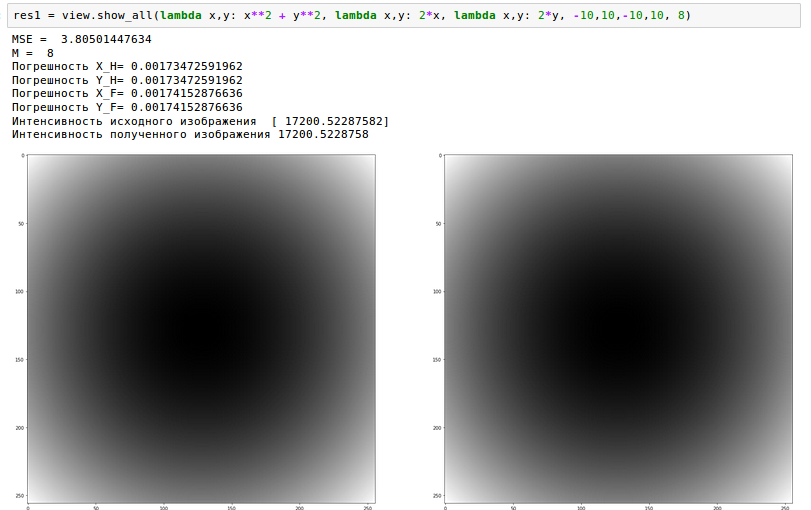
\includegraphics[width=1\linewidth]{R_2^2}}
\caption{Полином $R_2^2(x,y) = x^2 + y^2$}
\end{figure}

\begin{figure}
\center{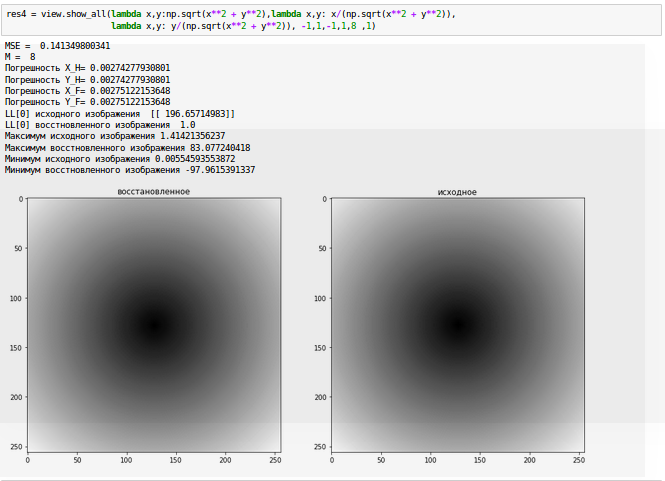
\includegraphics[width=1\linewidth]{R_1^1}}
\caption{Полином $R_1^1(x,y) = \sqrt{x^2 + y^2}$}
\end{figure}

\begin{figure}
\center{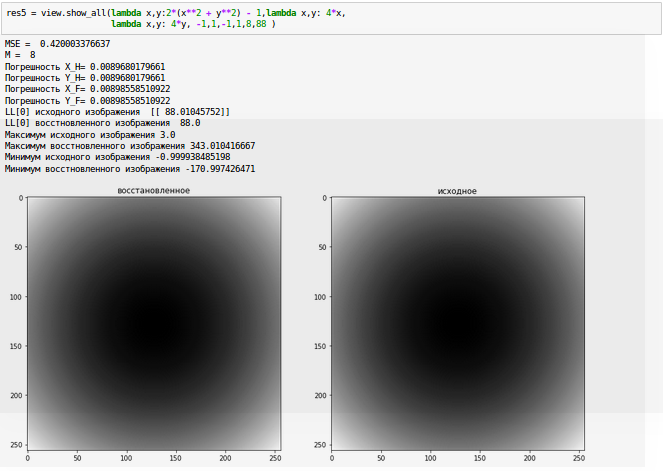
\includegraphics[width=1\linewidth]{R_2^0}}
\caption{Полином $R_2^0(x,y) = 2(x^2 + y^2) - 1$}
\end{figure}
\begin{figure}
\center{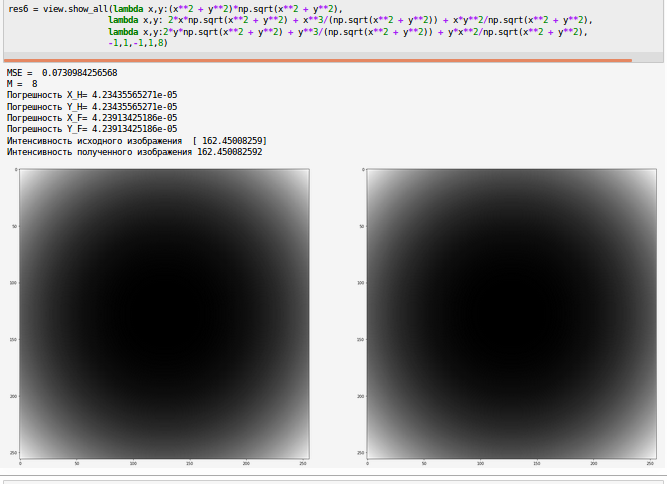
\includegraphics[width=1\linewidth]{R_3^3}}
\caption{Полином $R_3^3(x,y) = (x^2 + y^2)\sqrt{x^2 + y^2}$}
\end{figure}
\newpage
\section{Заключение}
В ходе работы удалось реализовать метод и проверить его работоспособность. Однако, реализовать именно тот алгоритм, который был предложен в \cite{new_method1} и \cite{new_method2} не удалось. Был использован менее эффективный по производительности алгоритм на основе формул для прямого преобразования. Были написаны модули для работы и исследования метода, с обособленной логикой, что позволит упростить дальнейшую разработку. Удалось инкапсулировать неоднозначную работу со сверткой сигналов и z-преобразованиями, и избежать конфликтов с модулем pywt, что может может в дальнейшем при тестировании. 

Из полученных программой результатов можно сделать вывод, что точность восстановления зависит от точности аппроксимации производной моделями Хаджина и Фрайда. Однако это требует дополнительных исследований.

Метод обладает ресурсом параллелизма ,а алгоритм возможно оптимизировать.
\newpage
\bibliography{bibl}

\end{document}